\chapter{อภิปรายผลลัพธ์ของโครงงาน}

\par{
    ภายหลังเสร็จสิ้นกระบวนการพัฒนาโครงงาน การทดสอบโครงงานและการนำเสนอแก่คณะกรรมการ ทางคณะผู้จัดทำได้รับผลตอบรับและข้อเสนอแนะจากทางคณะกรรมการที่น่าสนใจจำนวนหนึ่ง ซึ่งเหมาะสมแก่การนำมาอภิปรายและค้นหาแนวทางการปรับปรุงต่อได้ในอนาคต ซึ่งประกอบด้วยหัวข้อที่สำคัญ ดังนี้
}

\section{อภิปรายผลลัพธ์ของโมเดลปัญญาประดิษฐ์}
\subsection{ข้อคิดเห็นและข้อเสนอแนะจากคณาจารย์}
จากที่กล่าวไปข้างต้น ทางคณะผู้จัดทำได้รับข้อคิดเห็นจากคณะกรรมการ ดังนี้

\begin{enumerate}
    \item \textbf{ความน่าเชื่อถือของโมเดลปัญญาประดิษฐ์} : คณะกรรมการได้เล็งเห็นว่า การที่คณะผู้จัดทำได้มีการนำชุดข้อมูลมานิยามใหม่ (relabel) เพื่อนำอาชีพที่ใกล้เคียงกันมารวมเป็นสายอาชีพเดียวกัน อาจเป็นการกระทำที่เกิดมาจากความเห็นที่ไม่กลางของทางคณะผู้จัดทำโดยไม่รู้ตัวได้ และไม่มีข้อมูลหลักฐานใดยืนยันว่าความคิดนี้ถูกต้อง จึงเป็นจุดที่น่าวิเคราะห์ว่า โมเดลปัญญาประดิษฐ์นี้ จะมีความน่าเชื่อถือจากข้อมูลเหล่านี้ได้หรือไม่ ส่งผลให้คณะกรรมการเสนอว่า ทางคณะผู้จัดทำอาจต้องมีการเปลี่ยนแปลงวิธีการวัดผลความแม่นยำและน่าเชื่อถือของโมเดล
    \item \textbf{เมื่อคำนวณร่วมกับปัจจัยในข้อที่ผ่านมา การติดสินใจกลับไปใช้ rule-based อาจได้ผลลัพธ์ที่ดีกว่าหรือไม่} : 
    การที่คณะผู้จัดทำ เลือกมุ่งเน้นไปที่อัลกอริทึม TF-IDF ที่ใช้วิธีจับคำสำคัญของแต่ละสายอาชีพกับเรซูเมจากความถี่ ซึ่งคล้ายกับการใช้วิธีจับคู่คำกับเงื่อนไขโดยตรง (rule-based) จึงเกิดเป็นคำถามที่ว่า ทำไมเราถึงเลือกใช้โมเดลปัญญาประดิษฐ์ ทั้งที่ใช้ทรัพยากรสูงกว่า ทั้ง ๆ ที่ rule-based อาจมากเพียงพอแล้ว สำหรับการแก้ไขปัญหาด้วยการจับคู่เรซูเมกับสายงานด้วยคำสำคัญ
    
    ซึ่งทางคณะผู้จัดทำได้วางแผนเอาไว้ตั้งแต่แรกเริ่มแล้วว่า อยากทดลองพิสูจน์การใช้โมเดลปัญญาประดิษฐ์ ว่าจะสามารถให้ผลลัพธ์ที่ดีและแม่นยำกว่าได้หรือไม่ อย่างไรก็ตาม จากข้อความคิดเห็นของคณะกรรมการในข้อที่ 1 จึงเป็นลูกโซ่ให้เกิดข้อสงสัยว่าโมเดลปัญญาประดิษฐ์อาจไม่สามารถตอบโจทย์ได้หรือไม่
    
\end{enumerate}

\subsection{แนวทางการแก้ไขและแผนการดำเนินการ}
ทางคณะผู้จัดทำจึงคิดแนวทางการแก้ไขและปรับปรุงวิธีการวัดผลโมเดล เพื่อให้มีความน่าเชื่อถือมากขึ้น หรือมีแหล่งอ้างอิงที่เชื่อถือได้

\subsubsection{ทฤษฎี}
\textbf{การนิยามใหม่ (relabel)}

เพื่อทำให้การแบ่งสายอาชีพของชุดข้อมูลมีความน่าเชือถือ เราจึงออกแบบวิธีแก้ปัญหามา 2 แบบ ประกอบด้วย

\begin{enumerate}
    \item นำชุดข้อมูลที่เรามีไปพิสูจน์ต่อ โดยใช้ผู้เชี่ยวชาญจากงานด้านการบริหารทรัพยากรบุคคล (HR) มาช่วยเหลือในการตรวจสอบ แต่การให้ผู้เชี่ยวชาญมาตรวจสอบเรซูเมกว่า 200 เล่ม อาจส่งผลให้เกิดความเหนื่อยล้า ล่าช้า หรือความไม่เป็นกลางได้ ซึ่งจำเป็นต้องใช้ผู้เชี่ยวชาญจำนวนหลายคนเพื่อลดปริมาณงาน และตรวจสอบเรซูเมได้อย่างถูกต้องตามที่คาดหวัง อย่างไรก็ตาม วิธีการนี้ อาจเกิดอุปสรรคไม่รู้จบได้ นั่นคือ เราสามารถเชื่อถือ HR หรือบุคคลในสายงานเหล่านั้นได้หรือไม่
    \item ค้นหาชุดข้อมูลใหม่ โดยเราสามารถหาชุดข้อมูลใหม่ที่มีคุณภาพและเชื่อถือได้จากแหล่งที่เป็นที่ยอมรับหรือเป็นแหล่งที่ถูกใช้งานจริงโดยผู้ใช้ และมีการแบ่งสายอาชีพที่ถูกต้องอยู่แล้ว เราอาจต้องการขอความร่วมมือจากผู้ประกอบการหรือองค์กร เพื่อให้ได้ข้อมูลที่ถูกต้อง และน่าเชื่อถือ เช่น Jobsdb, JobThai หรือแพลตฟอร์มหางานต่าง ๆ อย่างไรก็ตาม วิธีการนี้ อาจมีอุปสรรคในเรื่องของการที่ต้องเตรียมวิธีการจัดการข้อมูลใหม่เองทั้งหมด    
\end{enumerate}

\textbf{การใช้โมเดลปัญญาประดิษฐ์ เปรียบเทียบกับ rule-based}

\par{
    เนื่องจาก rule-based เป็นวิธีที่เหมาะสมในบางสถานการณ์ เนื่องจากสามารถตั้งเงื่อนไขได้ตามต้องการ โดยที่วิธีการแก้ไขปัญหาปัจจุบันของคณะผู้จัดทำได้ใช้คำสำคัญในการแยกประเภทสายอาชีพ ซึ่งเราสามารถนำคำสำคัญเหล่านั้นมาตั้งเป็นเงื่อนไขได้เช่นกัน
}

\par{
    ซึ่งถ้าหากคณะผู้จัดทำสามารถตั้งเงื่อนไขได้ชัดเจนและครอบคลุม ก็จะเป็นวิธีในการแบ่งประเภทสายอาชีพที่มีประสิทธิภาพ รวมถึงไม่จำเป็นต้องใช้ทรัพยากรที่สูงด้วย
}

\par{
    อย่างไรก็ตาม ยังคงมีข้อเสียที่ควรพิจารณาร่วมด้วย เช่น การตั้งเงื่อนไขจะต้องครอบคลุมทั้งหมด และข้อจำกัดที่ไม่มีความยืดหยุ่น เนื่องจากเงื่อนไขที่ตั้งเอาไว้อาจจะไม่สามารถใช้ได้ในยุคสมัยที่เครื่องมือในการทำงานเปลี่ยนแปลงไปตลอดเวลา ไม่สามารถอัพเดทได้ทันทีจนกว่าจะมีการพัฒนาครั้งใหม่
}

\subsubsection{แผนการดำเนินการ}
\textbf{การนิยามใหม่ (relabel)}

\par{
    ทางคณะผู้จัดทำจะติดต่อขอความร่วมมือกับผู้ที่มีข้อมูลของผู้ที่ทำงานจริง เช่น Jobsdb ที่มีการเก็บรวบรวมเรซูเมของสายอาชีพต่าง ๆ เนื่องจากเป็นแพลตฟอร์มสมัครงานที่ใหญ่ และมีความน่าเชือถือที่สูง โดยที่ทางคณะผู้จัดทำจะส่งรายละเอียดของสายอาชีพที่ทางคณะผู้จัดทำแบ่งเอาไว้ 6 ประเภท เพื่อนำไปแบ่งสายอาชีพของเรซูเมที่ทางผู้ให้ความร่วมมือมี และส่งกลับมาเป็นชุดข้อมูลใหม่ต่อไป
}

\textbf{การใช้โมเดลปัญญาประดิษฐ์ เปรียบเทียบกับ rule-based}

\par{
    ทางคณะผู้จัดทำคิดพัฒนาระบบแบ่งสายอาชีพจากเรซูเม โดยใช้วิธีการแบบ rule-based เพื่อที่จะนำความแม่นยำมาเปรียบเทียบกับ KNN ที่ใช้อยู่ในปัจจุบันต่อไป 
}

\subsubsection{วิธีการวัดผล}
\textbf{การนิยามใหม่ (relabel)}

\par{
    เนื่องจากทางคณะผู้จัดทำจะนำชุดข้อมูลที่ถูกจัดประเภทมาจากทางองค์กรที่มีความน่าเชื่อถือและใช้งานอยู่จริง ทางคณะผู้จัดทำจึงคาดหวังว่าชุดข้อมูลเหล่านั้นจะเป็นชุดข้อมูลที่ใช้งานได้จริง
}

\textbf{การใช้โมเดลปัญญาประดิษฐ์ เปรียบเทียบกับ rule-based}

\par{
    เมื่อทางคณะผู้จัดทำได้พัฒนาเครื่องมือในการทำนายสายอาชีพด้วย rule-based แล้ว เราจะนำ Accuracy score และ Confusion Matrix มาเปรียบเทียบกับ KNN ที่ใช้อยู่ในปัจจุบัน เพื่อดูว่ามีความถูกต้องอยู่ที่เท่าไหร่ และในกรณีที่ไม่ถูกต้อง มักจะทำนายไปในสายอาชีพใด
}

\par{
    โดยคณะผู้จัดทำก็จะใช้วิธีการวัดผลแบบเดียวกับ KNN คือนำเรซูเมไปทำการทดลองแบบอำพราง (Blind Test) กับผู้เชี่ยวชาญในสายงานเหล่านั้นต่อไป
}

\par{
    หากวิธีการแบบ rule-based สามารถให้ผลลัพธ์ที่ดีกว่า หลังจากโมเดล KNN ผ่านการวิเคราะห์ใหม่แล้ว อาจบอกได้ว่า การใช้ rule-based อาจยังมีประสิทธิภาพกว่า และโมเดลปัญญาประดิษฐ์ของเราถือว่ายังไม่ตอบโจทย์
}

\subsection{แนวทางในอนาคต และข้อคิดเห็นจากทีมงาน}

\par{
    จากวิธีการแก้ปัญหาที่คณะผู้จัดทำวางแผนไว้ ทางเราคาดหวังว่าชุดข้อมูลเรซูเม และสายอาชีพที่ได้รับมาจากการขอความร่วมมือกับทางองค์กรที่ให้บริการเกี่ยวกับการสมัครงานจะมีความน่าเชือถือ และสมบูรณ์ ซึ่งจะเป็นหนึ่งในส่วนสำคัญที่จะสามารถทำให้ระบบทำนายสายอาชีพมีความแม่นยำต่อไป
}
\par{
    นอกจากนี้ คณะผู้จัดทำยังคงยืนยันว่า rule-based เหมาะสมกับชุดข้อมูลที่ไม่ได้เปลี่ยนแปลงบ่อย ซึ่งเครื่องมือการทำงานของแต่ละสายอาชีพอาจจะมีการเปลี่ยนแปลงตามกาลเวลา ส่งผลให้การที่จะคงข้อดีของ  rule-based เอาไว้ในระยะยาวอาจจะเป็นสิ่งที่ยากกว่า KNN ที่สามารถปรับตัวกับชุดข้อมูลใหม่ ๆ ได้ง่ายกว่าผ่านการนำมาเทรนต่อ

}
\par{
    อย่างไรก็ตาม ทางคณะผู้จัดทำไม่สามารถปฏิเสธได้เลยว่า หากมีการดำเนินการทดสอบแก้ไขโมเดลปัญญาประดิษฐ์ตามแผนที่วางไว้ และผลลัพธ์ในท้ายประบวนการมีผลที่ต่ำกว่าเดิมจากเกณฑ์การวัดใหม่ของเราและต่ำกว่าการใช้ rule-based โดยตรง ก็อาจสามารถบอกได้ว่า การใช้โมเดลปัญญาประดิษฐ์อาจยังไม่ตอบโจทย์ได้ตามที่คณะกรรมการคาดเดาไว้ ซึ่งหมายความว่า ในส่วนของโมเดลปัญญาประดิษฐ์ของเรา อาจยังไม่สามารถบรรลุได้ตามเป้าหมายนั่นเอง
}







\section{อภิปรายผลลัพธ์ของเว็บแอปพลิเคชัน}
\subsection{ข้อคิดเห็นและข้อเสนอแนะจากคณาจารย์}
ในส่วนของเว็บแอปพลิเคชัน เราได้ข้อแนะนำจากคณะกรรมการ ดังนี้

\begin{enumerate}
    \item \textbf{ความน่าเชื่อถือในการวัดผลและความสำเร็จ} : แม้ว่าทางคณะผู้จัดทำจะทำการเก็บผลสำรวจและทดสอบโครงงานมาก่อนแล้ว อย่างไรก็ตาม คณะกรรมการเล็งเห็นว่า ควรจะมีการวัดผลในระยะยาวด้วยหรือไม่ นอกเหนือจากความพอใจระยะสั้น ซึ่งคณะกรรมการเองก็มีข้อกังวลเช่นกัน เพราะเป็นสิ่งที่ไม่สามารถวัดผลได้แน่ชัด จึงฝากฝังให้คณะผู้จัดทำทดลองนำหัวข้อดังกล่าวกลับมาประเมินอีกครั้ง
    \item \textbf{ลักษณะการใช้งานที่อาจนำไปสู่การชี้แนวทางสายอาชีพแบบบังคับได้} : ลักษณะการใช้งานเว็บแอปพลิเคชันในปัจจุบัน จะให้ผู้ใช้ทำการกรอกข้อมูลเรซูเมของตนเอง และปัญญาประดิษฐ์จะทำการวิเคราะห์ผลลัพธ์กลับไปให้ ซึ่งลักษณะการใช้งานเช่นนี้ คณะกรรมการได้มองว่า เป็นเหมือนการบอกบังคับทางอ้อมว่าผู้ใช้งานควรจะเข้าสู่สายอาชีพแบบใด ถึงแม้ว่าจะมีระบบการเปรียบเทียบความสามารถเพื่อช่วยเหลือการชี้แนะที่ดีขึ้นแล้วก็ตาม จึงเป็นโจทย์ที่ทางคณะผู้จัดทำควรคิดวิธีการแก้ไข เพื่อให้โครงงานเป็นไปตามที่คาดหวังและวางจุดประสงค์เอาไว้ นั่นคือ การแนะนำแนวทางการเรียนรู้และปรับปรุงเรซูเม ไม่ใช่การตัดสินเรซูเมและชี้แนะแกมบังคับ
\end{enumerate}

\subsection{แนวทางการแก้ไขและแผนการดำเนินการ}
ทางคณะผู้จัดทำจึงตัดสินใจออกแบบแนวทางการวัดผลที่อาจช่วยในการวัดผลของโครงงานในระยะยาว และออกแบบวิธีการแก้ไขเพื่อปรับปรุงวิธีการใช้งานให้ดีขึ้น ดังนี้

\begin{enumerate}
    \item \textbf{วิธีการวัดผลระยะยาว}
    
    \par{
        จากจุดประสงค์เริ่มแรกของทางคณะผู้จัดทำ เราไม่ได้ครอบคลุมไปถึงการวัดผลระยะยาวด้วย เนื่องจากเป็นสิ่งที่วัดผลได้ไม่แน่นอน เปลี่ยนแปลง และผันผวนได้ง่าย อย่างไรก็ตาม หากเป็นเกณฑ์ที่เกี่ยวเนื่องกับเกณฑ์ในปัจจุบัน ทางเรามองว่า สามารถทำได้ และยังสามารถวัดผลได้ตามที่คาดการณ์ไว้ โดยเราแบ่งเป็นเกณฑ์ต่าง ๆ ดังนี้
    }


    \textbf{ประสิทธิภาพในการเขียนเรซูเม}


    \begin{itemize}
        \item วัดระยะเวลาเฉลี่ยที่ผู้ใช้ใช้ในการสร้างเรซูเมก่อนและหลังใช้เว็บไซต์
        \item เปรียบเทียบข้อมูลภายในเพื่อประเมินการลดลงของเวลาที่ใช้ ซึ่งบ่งชี้ถึงประสิทธิภาพในการทำเรซูเมที่เพิ่มขึ้นภายหลังการใช้เว็บไซต์
    \end{itemize}

    \textbf{ประสิทธิผลของการสมัครงาน}


    \begin{itemize}
        \item เก็บข้อมูลจำนวนการตอบกลับและการเชิญสัมภาษณ์ที่ผู้ใช้ได้รับ
        \item คำนวณอัตราการตอบรับต่อการสมัครงานเพื่อวัดประสิทธิผลของเรซูเมที่สร้างภายหลังจากใช้งานเว็บไซต์
    \end{itemize}

    \textbf{อัตราความสำเร็จในการสมัครงาน}


    \begin{itemize}
        \item ติดตามจำนวนการสมัครงานที่ประสบความสำเร็จของผู้ใช้ก่อนและหลังใช้เว็บไซต์
        \item วิเคราะห์การเปลี่ยนแปลงของอัตราความสำเร็จเพื่อประเมินผลเว็บไซต์ต่อคุณภาพของเรซูเม
    \end{itemize}

    \textbf{ความมั่นใจของผู้สมัคร}


    \begin{itemize}
        \item ดำเนินการสำรวจความคิดเห็นก่อนและหลังการใช้งานเว็บไซต์
        \item ใช้มาตรวัด Likert scale เพื่อประเมินระดับความมั่นใจในโปรไฟล์และเรซูเมของผู้ใช้
    \end{itemize}

    \item \textbf{วิธีการแก้ไขการใช้งานที่อาจชี้นำผู้ใช้จนเกินไป}
    
    \par{
        เปลี่ยนรูปแบบการจัดวางส่วนประสานผู้ใช้ (user interface) ให้เป็นมิตรแก่การชี้แนะมากขึ้น เช่น การเปิดโอกาสให้ผู้ใช้เลือกสายอาชีพที่ต้องการแต่แรกเริ่ม เพื่อลดการชี้แนะโดยไม่ได้ตั้งใจ วิธีนี้ จะเป็นการมอบอำนาจการควบคุมเว็บไซต์ให้แก่ผู้ใช้ทั้งหมด อาจส่งผลให้ผู้ใช้ต้องเรียนรู้เว็บไซต์นานขึ้น แต่จะทำให้ผู้ใช้สามารถใช้งานได้โดยไม่ถูกชี้นำโดยผู้จัดทำ
    }

    โดยทางเราได้ออกแบบ user interface ที่ถูกแก้ไขเอาไว้ตามแผนเอาไว้ ดังนี้

    \begin{figure}[H]\centering
        \fbox{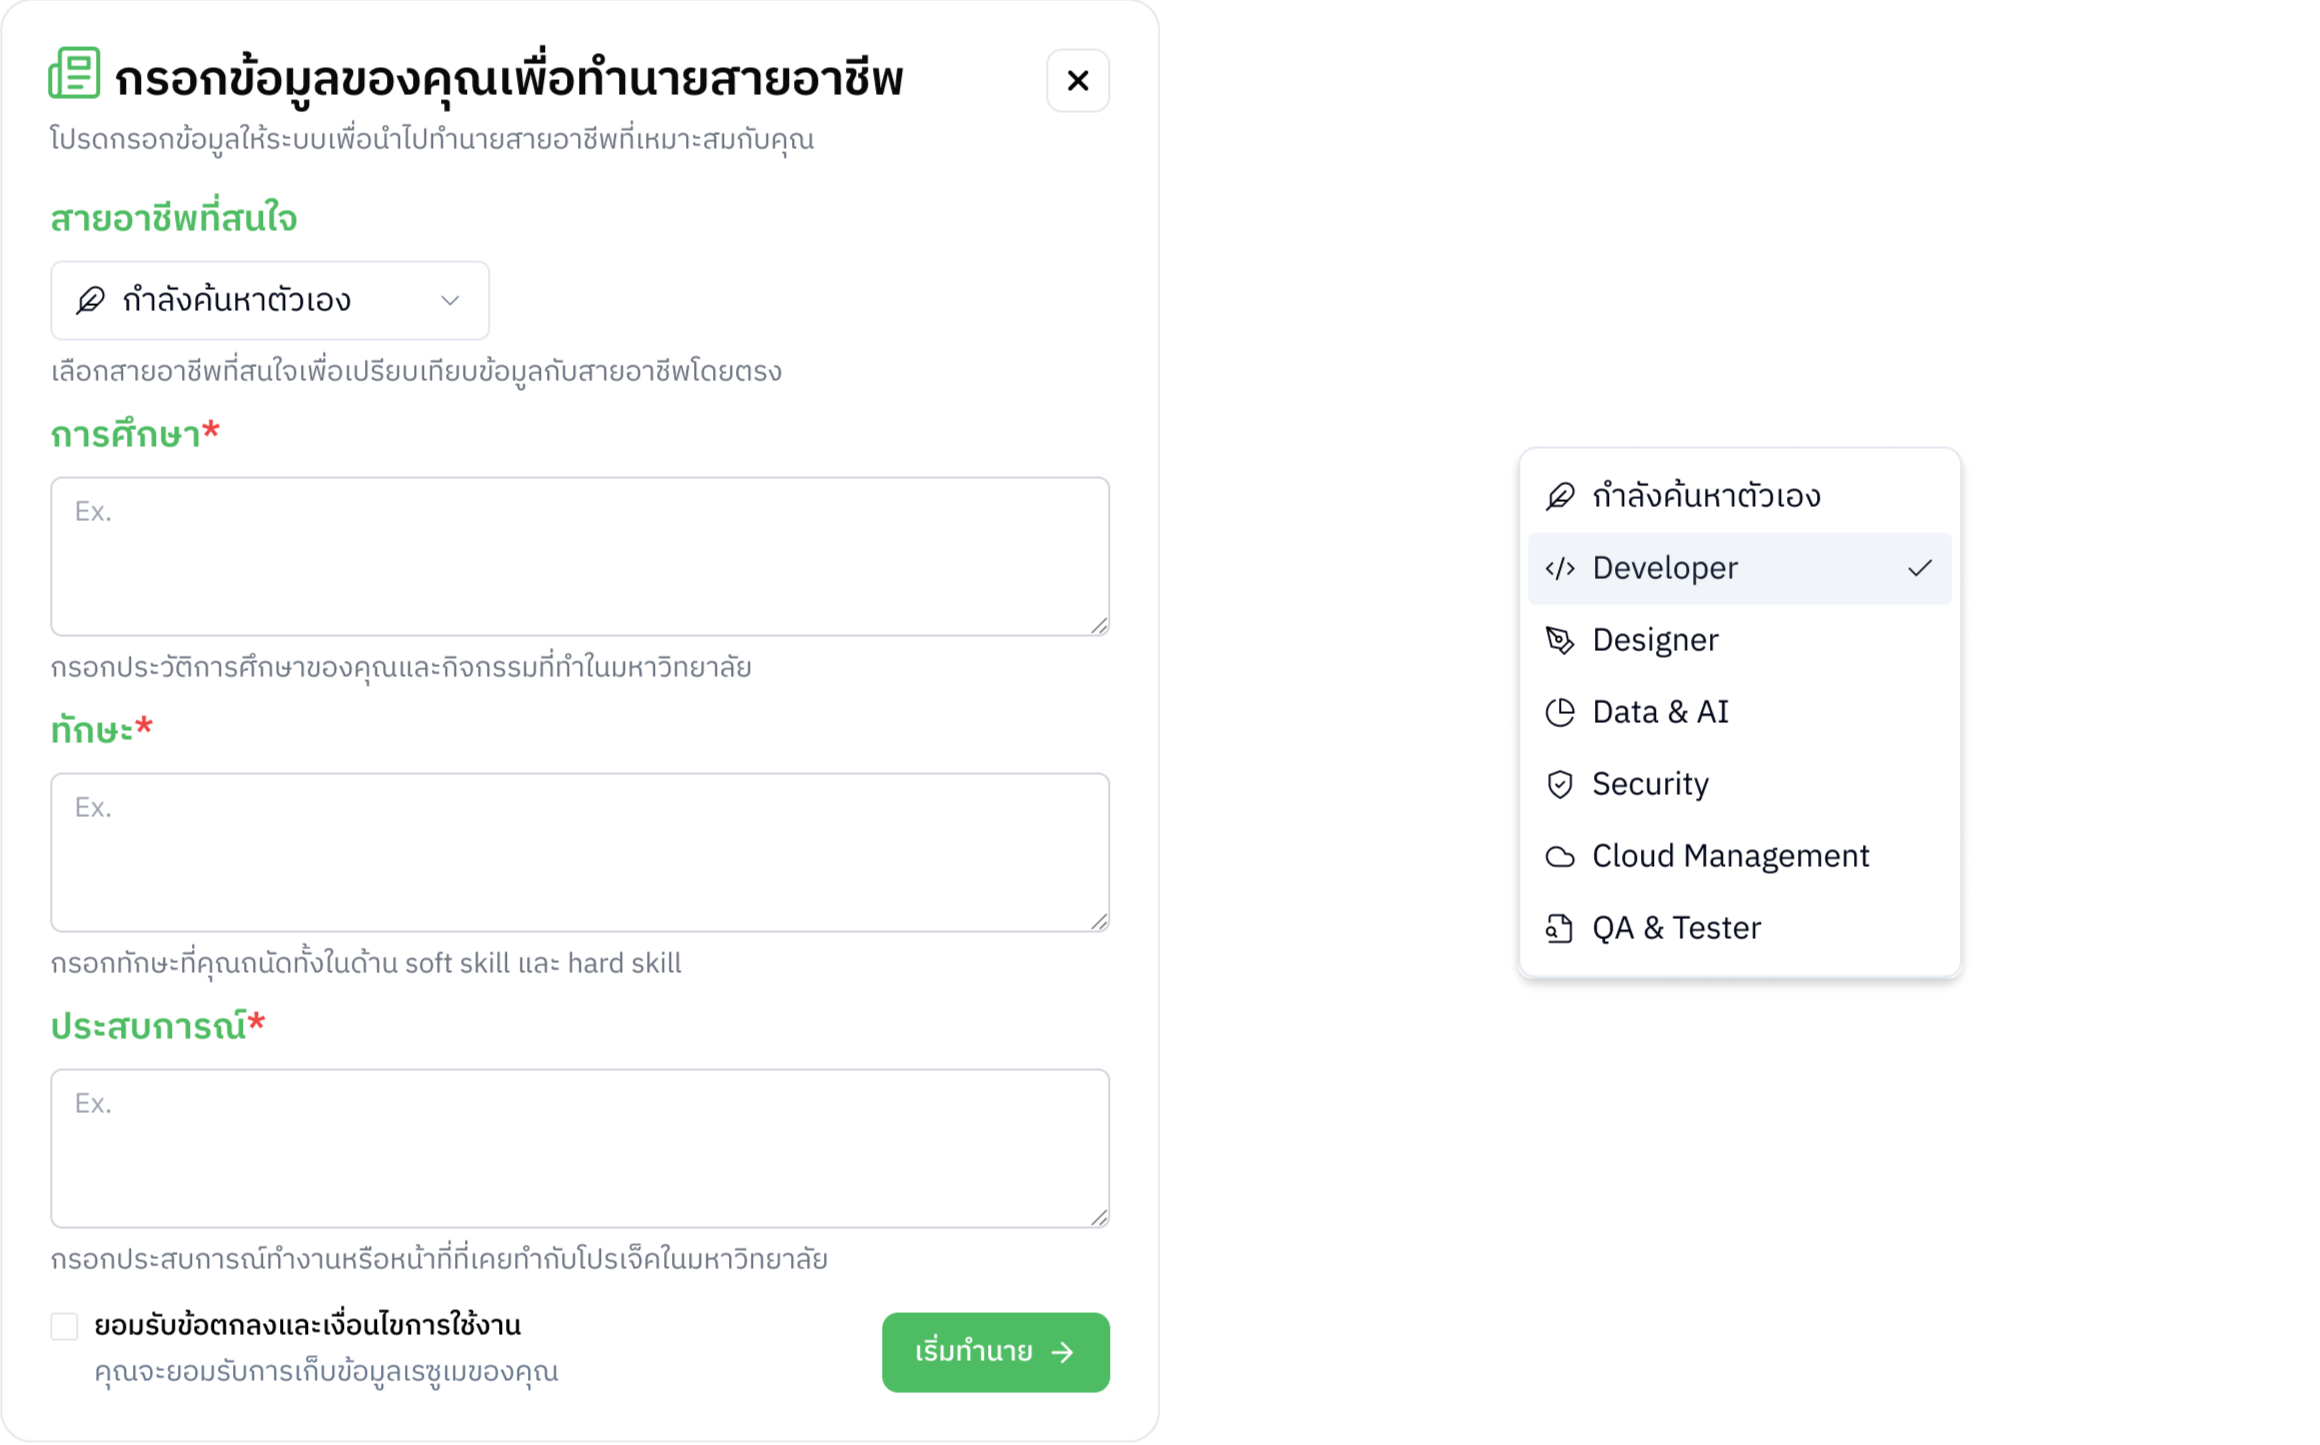
\includegraphics[width=10cm]{./figure/figure_new_ui.jpg}}
        \caption{รูปแสดงตัวอย่างการแก้ไขส่วนประสานผู้ใช้ใหม่}\label{fig:new-ui}
    \end{figure}

\end{enumerate}


\subsection{แนวทางในอนาคต และข้อคิดเห็นจากทีมงาน}

\par{
    จากแผนการดำเนินการที่เราคิดค้นขึ้น หากมีโอกาสได้ทดลองเก็บผลลัพธ์และพัฒนาเพิ่มเติมแล้ว อาจส่งผลให้เราต้องทำการปรับปรุงการออกแบบใหม่เพื่อมอบประสบการณ์ที่ดีขึ้นให้แก่ผู้ใช้ ซึ่งสามารถทำให้สำเร็จได้หากมีเวลาและโอกาส อย่างไรก็ตาม การวัดผลในบางกรณีอาจทำได้ยาก เช่น การวัดผลในระยาว เพราะมีปัจจัยจำนวนมากที่ส่งผลถึงตัวผู้ใช้ ทำให้การวัดผลเกิดความคลาดเคลื่อนได้ง่าย ดังนั้น อาจต้องยอมรับว่า การวัดผลในกรณีเช่นนี้ อาจต้องย้อนกลับไปที่จุดประสงค์แรกเริ่มของพวกเรา คือ ความพึงพอใจของผู้ใช้
}